This section contains the main problem for this project and the form of solution required.
Further the scope and the limitations also are defined here.
\subsection{The problem}
The basis of this project is Aalborg Bycyklen \cref{aalborg_bycyklen}.
The challenges that are described in \cref{aalborg_bycyklen:challenges} are the one that needs being solved.
The main problems being:
\begin{itemize}
\item Improve flexibility
\item Improve reliability
\item Find lost bikes
\item Repairment of bikes
\end{itemize}

\subsection{Solution}
The biggest change to the current system, will be the addition of GPSs in the bikes.
This will bring the following changes:
\begin{itemize}
\item It will be possible to track the position of bikes.
\item Bike stations will be completely obsolete, \bruno{Giovanni: "Why? CPH uses bike stations even though it uses GPS."} instead 'hot-spots' will be introduced.
\item It will be possible to monitor the usage of bikes and make statistical predictions on future locations.
\end{itemize}

\paragraph{Bike stations are unnecessary}
So far, bike stations serve a limited purpose.
They are where people are supposed to place the bikes after use, thus making it possible for other people to find the bikes.
However, bikes are not necessarily returned to a station after use, somewhat disrupting the sole purpose of the bike stations.

\paragraph{GPS}
Furthermore, by adding GPSs to the bikes, it will be possible to get an exact location of a bike, even if it is not at a bike station.
By monitoring the location of the bikes, their movements could be tracked.
Further, by detecting long stops (meaning ended trip), so-called hot-spots could be determined.

\paragraph{Hot-spot}
A hot-spot is an area, like an informal station.
But hot-spots come and go, depending on the use of the bikes.
A hot-spot is initialized when several bikes are available at the hot-spot location.
This is determined by looking at the history of the bike usage.

\paragraph{Locating bikes}
By requesting GPS locations on bikes, it will be possible to get an overview of all bikes.
The system may select an available bike nearby and guide the user to its location.
It can also be used by Aalborg Kommune, to locate missing or stolen bikes.

In regards to users locating bikes, they should have a more limited view, as compared to Aalborg Kommune.
They should be restricted to viewing bikes that are available and nearby.
As of now, it is not completely certain how a bike will be confirmed available, but the main idea is to do so after a given period of time with no activity.\bruno{Giovanni: "Can you elaborate on that? Possible questions: log-in/out system like in CPH? What is a reasonable period of time?"}

If a bike should leave the Aalborg area, Aalborg Kommune should be notified.
If a bike is inactive for too long, it could mean that it is broken or parked too far away for anyone to use it.
Then Aalborg Kommune could be notified, and someone can be sent to either make repairs or move it.

\paragraph{Structure of the solution}
\bruno{Description}
The structure of the solution can be seen on \cref{fig:solution_structure}.

\begin{figure}
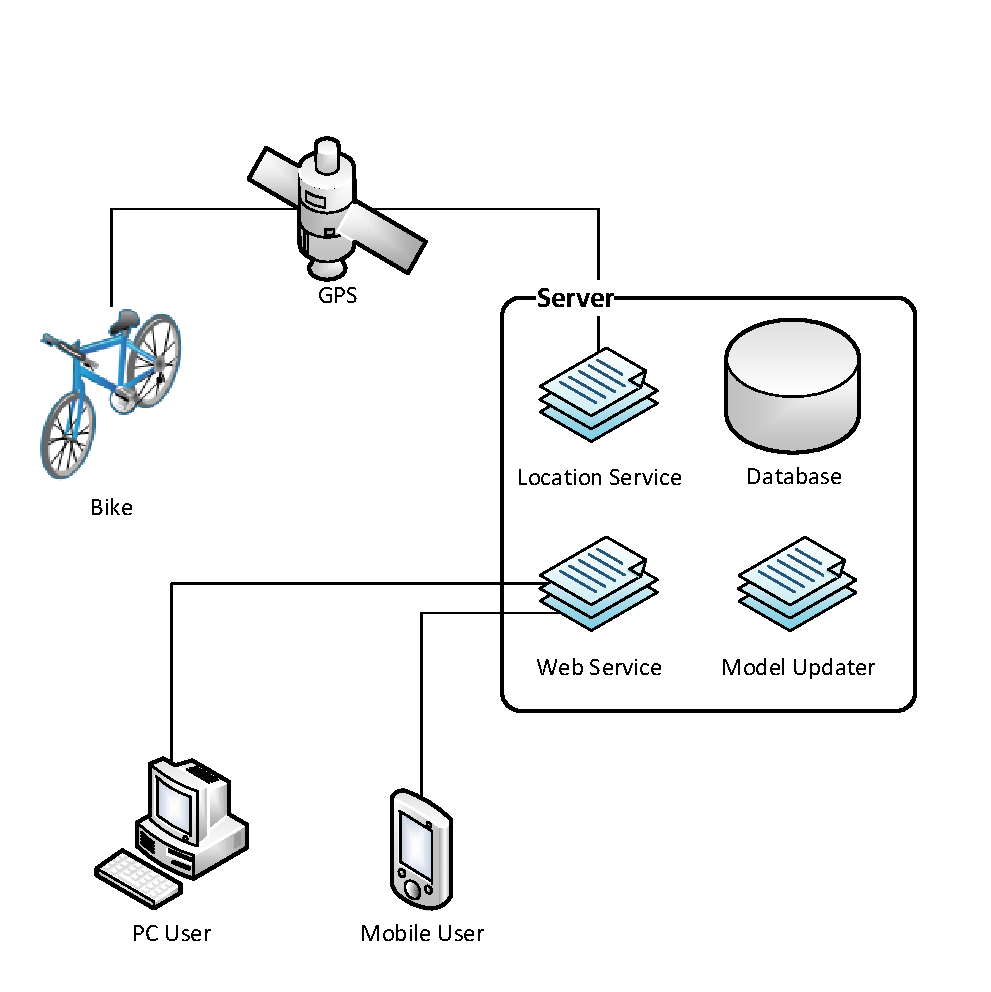
\includegraphics[width=\textwidth]{our_solution.pdf}
\caption{The overall structure of our solution}
\label{fig:solution_structure}
\end{figure}

\subsection{Limitations}
The limits presented in the list below:
\begin{itemize}
\item Time: The project is due the [insert due date]
\item There are not provided any money for the project
\end{itemize}

\subsection{Scope}
Because of the limitations mentioned above this project will be developing a webservice, a location service and an agent system.
Which can be seen on \cref{fig:solution_structure} in the blue box.
